\documentclass[11pt,a4paper]{article}
\usepackage{tikz}
\usetikzlibrary{arrows.meta,positioning}
\usepackage{tabularx}
\usepackage{amsmath,amssymb,amsthm}
\usepackage{geometry}
\geometry{margin=1in}
\usepackage{hyperref}
\usepackage{graphicx}
\usepackage{setspace}
\onehalfspacing

\title{\textbf{Paper A-05: Earth Soil Pedogenesis:\\ A Constraint-Driven Flux Dynamics (CDFD) Perspective}}
\author{Steve Bico Mujjabi, MD\\
\small Independent Researcher\\
\small Founder, Vura Labs\\
\small Kampala, Uganda\\
\small ORCID: 0009-0001-0556-5516}
\date{August 2026}

\begin{document}
\maketitle

% BEGIN SHARED-METHODS POINTER
\noindent\textit{Shared Part IV notation and evidence boundaries are defined in \path{PART_IV_METHODS_AND_CLAIM_BOUNDARY.md}. This paper states only its local observables, comparison, and failure conditions.}
% END SHARED-METHODS POINTER


\begin{abstract}
This paper develops a falsifiable CDFD/AFL model of Earth Soil Pedogenesis. It maps weathering, water, organic inputs, roots, and land-use pressure to driving flux $\Phi$, porosity, nutrient limitation, mineralogy, and erosion to active constraint $C$, aggregation, bioturbation, root growth, and microbial turnover to responsiveness $S$, and compaction, contamination, horizon development, and carbon legacy to structural memory $M_s$. The target outcome is infiltration, fertility, carbon retention, and erosion resistance, tested against soil profiles, long-term field trials, spectroscopy, infiltration tests, and carbon records. The paper treats universality as a shared model architecture rather than an assertion that unlike systems have the same material mechanism. It states the negative result that would make the mapping unnecessary and places the domain claim inside the cumulative CDFD programme and its reproducible runtime boundary.
\end{abstract}

\section{Introduction}

Topsoil is the most valuable and fragile energetic membrane on Earth. It is a highly complex, porous structure built by the relentless biological labor of fungi, bacteria, and plant roots breaking down solid rock constraint into bioavailable fluid flux.

When humans engage in industrial agriculture, they aggressively manipulate this membrane. CDFD reveals that soil is subject to comparable finite-capacity boundaries as human physiology. You cannot infinitely extract flux from a membrane without structurally damaging its constraints and memory.

\section{The Pedological Adaptive Surface}
We evaluate the health of a soil horizon using the Adaptive Operating Ratio:
\begin{equation}
    \Psi_s = \left( \frac{\Phi}{C} \right) \cdot S \cdot M_s
\end{equation}

For a specific plot of land:
\begin{itemize}
    \item \textbf{Flux ($\Phi$)}: The throughput of water, carbon, nitrogen, and phosphorus moving through the soil profile, driven by plant uptake and microbial metabolism.
    \item \textbf{Constraint ($C$)}: The physical bedrock impermeability, soil compaction, and the scarcity of base minerals.
    \item \textbf{Responsiveness ($S$)}: The porosity and organic matter content of the soil, determining its ability to absorb and hold water and nutrients (cation exchange capacity).
    \item \textbf{Memory ($M_s$)}: The highly complex, specialized mycelial networks and microbiome communities that have taken centuries to establish. This biological memory locks the soil into a highly efficient nutrient-routing topology.
\end{itemize}

\subsection{Desertification and Topological Death}
A healthy, untouched prairie exists at $\Psi_s \approx 1$. The deep root systems and fungal networks (high $M_s$) perfectly manage the heavy rain flux ($\Phi$) and the bedrock constraints ($C$).

Introduce industrial tilling and heavy chemical fertilization. The physical tilling violently destroys the mycelial networks---an instantaneous, total erasure of the system's structural memory ($M_s \to 0$). Simultaneously, heavy tractors increase soil compaction, drastically raising the physical constraint $C$.

When root, pore, and fungal structure are damaged, effective responsiveness $S$ may fall. Under heavy rain, reduced infiltration can increase runoff and erosion. The CDFD claim is limited to a measurable history-dependent soil response; comparison with an ischemic organ is an analogy, not a shared material mechanism.



\section{Measurement Layer}

% BEGIN PART IV MAJOR CROSS-DOMAIN UPGRADE
\section{Cross-Domain Model Upgrade: Mechanism, Scale, and Tests}

\subsection{Observable Translation}

The paper-specific translation begins with an observable chain rather than a
verbal analogy. For Earth Soil Pedogenesis, the proposed drive is weathering, water, organic inputs, roots, and land-use pressure.
The active limitation is porosity, nutrient limitation, mineralogy, and erosion. Responsiveness is carried by
aggregation, bioturbation, root growth, and microbial turnover, while retained state is represented by
compaction, contamination, horizon development, and carbon legacy. The outcome to explain is infiltration, fertility, carbon retention, and erosion resistance.

\begin{table}[htbp]
\centering
\small
\caption{Operational CDFD/AFL map for Paper A-05.}
\begin{tabularx}{\textwidth}{|l|X|X|}
\hline
\textbf{Term} & \textbf{Paper-specific observable meaning} & \textbf{Measurement question} \\
\hline
$\Phi$ & weathering, water, organic inputs, roots, and land-use pressure & What rate, load, gradient, or demand enters the focal system? \\
\hline
$C$ & porosity, nutrient limitation, mineralogy, and erosion & Which measured bottleneck limits transfer, function, or recovery? \\
\hline
$S$ & aggregation, bioturbation, root growth, and microbial turnover & Which process changes effective capacity or reroutes the load? \\
\hline
$M_s$ & compaction, contamination, horizon development, and carbon legacy & Which retained state makes equal present loads produce different futures? \\
\hline
$Y$ & infiltration, fertility, carbon retention, and erosion resistance & Which outcome is predicted out of sample, with uncertainty? \\
\hline
\end{tabularx}
\end{table}

\begin{figure}[htbp]
\centering
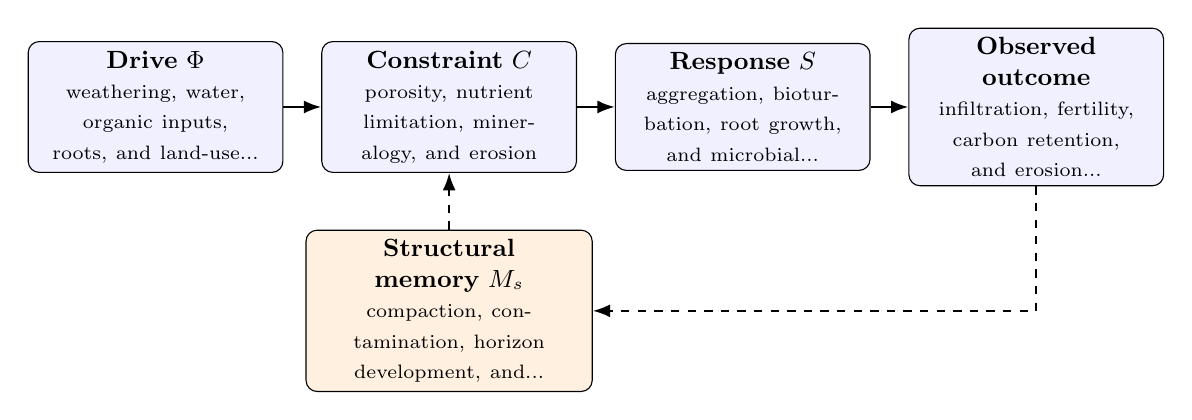
\begin{tikzpicture}[
    node distance=0.48cm,
    every node/.style={font=\small},
    box/.style={draw, rounded corners, align=center, minimum height=1.45cm, text width=3.0cm, fill=blue!6},
    memory/.style={draw, rounded corners, align=center, minimum height=1.25cm, text width=3.4cm, fill=orange!12},
    flow/.style={-{Latex[length=2.2mm]}, thick},
    feedback/.style={-{Latex[length=2.2mm]}, thick, dashed}
]
\node[box] (drive) {\textbf{Drive $\Phi$}\\\scriptsize weathering, water, organic inputs, roots, and land-use...};
\node[box, right=of drive] (constraint) {\textbf{Constraint $C$}\\\scriptsize porosity, nutrient limitation, mineralogy, and erosion};
\node[box, right=of constraint] (response) {\textbf{Response $S$}\\\scriptsize aggregation, bioturbation, root growth, and microbial...};
\node[box, right=of response] (outcome) {\textbf{Observed outcome}\\\scriptsize infiltration, fertility, carbon retention, and erosion...};
\node[memory, below=0.72cm of constraint] (memory) {\textbf{Structural memory $M_s$}\\\scriptsize compaction, contamination, horizon development, and...};
\draw[flow] (drive) -- (constraint);
\draw[flow] (constraint) -- (response);
\draw[flow] (response) -- (outcome);
\draw[feedback] (outcome.south) |- (memory.east);
\draw[feedback] (memory.north) -- (constraint.south);
\end{tikzpicture}
\caption{Paper A-05 observable CDFD/AFL architecture for Earth Soil Pedogenesis. Solid arrows give the proposed forward chain; dashed arrows make history-dependent feedback explicit.}
\label{fig:a05-architecture}
\end{figure}

\subsection{Paper-Specific Causal Hypothesis}

For this paper, the hypothesized causal sequence is specific. A change in
weathering, water, organic inputs, roots, and land-use pressure arrives faster than aggregation, bioturbation, root growth, and microbial turnover can compensate.
This raises or redistributes porosity, nutrient limitation, mineralogy, and erosion. If the load persists,
the retained state encoded by compaction, contamination, horizon development, and carbon legacy changes the next response, so a later event of equal
magnitude can produce a different trajectory in infiltration, fertility, carbon retention, and erosion resistance. The
scientific task is to estimate that sequence against the best ordinary model of
the domain, not merely to redescribe the outcome after it occurs.

\subsection{Cross-Scale Translation Without Mechanistic Erasure}

For the Earth systems family, the cross-domain translation compares coupled transport, finite environmental capacity, buffering, and retained landscape or ecosystem state. It cannot erase conservation laws, geometry, or scale; it must expose where those domain equations create comparable overload and recovery structures. \cite{Holling1973,Turing1952,BakTangWiesenfeld1987}
The required scale declaration for this paper is days to millennia; aggregates to landscapes. At short
scales, the key question is whether the incoming drive is transmitted,
buffered, or diverted. At intermediate scales, response changes effective
capacity and network exposure. At long scales, retained structure can alter the
state space itself. A result is genuinely cross-scale only when the aggregation
rule is stated and the same conclusion is not an artifact of averaging.

\subsection{Evidence Ladder and Discriminating Tests}

\begin{table}[htbp]
\centering
\small
\caption{Evidence ladder for Paper A-05. Each rung can fail independently.}
\begin{tabularx}{\textwidth}{|p{0.17\textwidth}|X|X|}
\hline
\textbf{Test} & \textbf{Design} & \textbf{Discriminating result} \\
\hline
Proxy audit & Measure soil profiles, long-term field trials, spectroscopy, infiltration tests, and carbon records and preregister how each record maps to $\Phi$, $C$, $S$, $M_s$, and $Y$. & The mapping fails if proxies are non-identifiable, circular, or change meaning across cases. \\
\hline
Load ramp & Apply or observe repeated cultivation or drought followed by restoration while estimating the dominant constraint and response time. & A threshold claim requires a reproducible nonlinear change and uncertainty bounds, not a visually chosen breakpoint. \\
\hline
Recovery and memory & Match present load across units with different histories, then compare recovery paths. & The memory claim requires history-dependent divergence after current conditions are controlled. \\
\hline
Model comparison & Compare the baseline domain model with and without the CDFD/AFL state variables using held-out data. & The paper's stated falsifier is: soil recovery is independent of prior-load history after controlling for present conditions. \\
\hline
\end{tabularx}
\end{table}

\subsection{Research Programme and Boundary Conditions}

The immediate research programme has four steps. First, construct a documented
dataset from soil profiles, long-term field trials, spectroscopy, infiltration tests, and carbon records and retain raw units before normalization.
Second, fit a baseline domain model and report its calibration and out-of-sample
error. Third, add the smallest identifiable CDFD/AFL state extension and test
whether it improves prediction of infiltration, fertility, carbon retention, and erosion resistance. Fourth, repeat the
analysis across the declared scale range and publish negative cases as part of
the cross-domain translation audit.

% END PART IV MAJOR CROSS-DOMAIN UPGRADE

\section{Conclusion}
Dirt is dead; soil is alive. By treating pedogenesis through the lens of CDFD, we see that soil is a living thermodynamic membrane requiring structural memory and low constraint to function. Sustainable agriculture is not merely an ecological preference; it is the physical necessity of maintaining a mathematically stable $\Psi_s$ across the Earth's primary biological interface.
\section*{Conflict of Interest} The author declares no conflict of interest.
\section*{Data Availability}
Part-specific runtime diagnostics are under each Part's \path{outputs/} directory.

Release-wide code: \path{Part_E_Synthesis/supplementary/}.

Generated summaries: \path{Part_E_Synthesis/outputs/}.

Figures: \path{Part_E_Synthesis/figures/}.


\section{Reference Layer}
\bibliographystyle{plain}
\bibliography{universal_afl_references}
\end{document}
